\chapter{Der Allgemeine Workflow in TensorFlow}





\section{Die Tooling Pipeline}



\section{Vorgehensweise beim Trainingsprozess}

\newpage



\section{Die Visualisierung mit TensorBoard}

TensorBoard ist eine in der Installation von TensorFlow enthaltene Webanwendung zur Visualisierung der Abläufe in einem neuronalen Netz. TensorBoard stellt eine Vielzahl an graphischen Elementen zur Verfügung, welche dem Entwickler vorallem das Debuggen oder die Optimierung eines erstellten Modells erleichtern. Ebenso können damit insbesondere komplexe Datenstrukturen zum besseren Verständnis anschaulich visualisiert werden.

Bevor mit TensorBoard gearbeitet werden kann, muss folgender Befehl \ref{formel1} in die Kommandozeile eingegeben werden:
\\

\begin{equation}
\displaystyle tensorboard\quad--logdir=path/to/log\_directory
\label{formel1}
\end{equation}

\vspace{0.4cm}
wobei vorher im spezifizierten Log Ordner die gewünschten Event Daten mit der Klasse \textit{tf.summary.FileWriter('path/to/log-directory')} abgespeichert werden müssen. Nachdem TensorBoard gestart wurde, navigiert man mit dem Browser zu folgender Seite:


\begin{equation}
\displaystyle http://localhost:6006
\label{formel2}
\end{equation}

Falls keine Fehlermeldungen aufgetreten sind, sollte folgender Bildschirminhalt angezeigt werden:
\\[1ex]

\begin{figure}[h!]
	\centering
	%\vspace{-35pt}
	%\hspace{-1.0cm} 
	 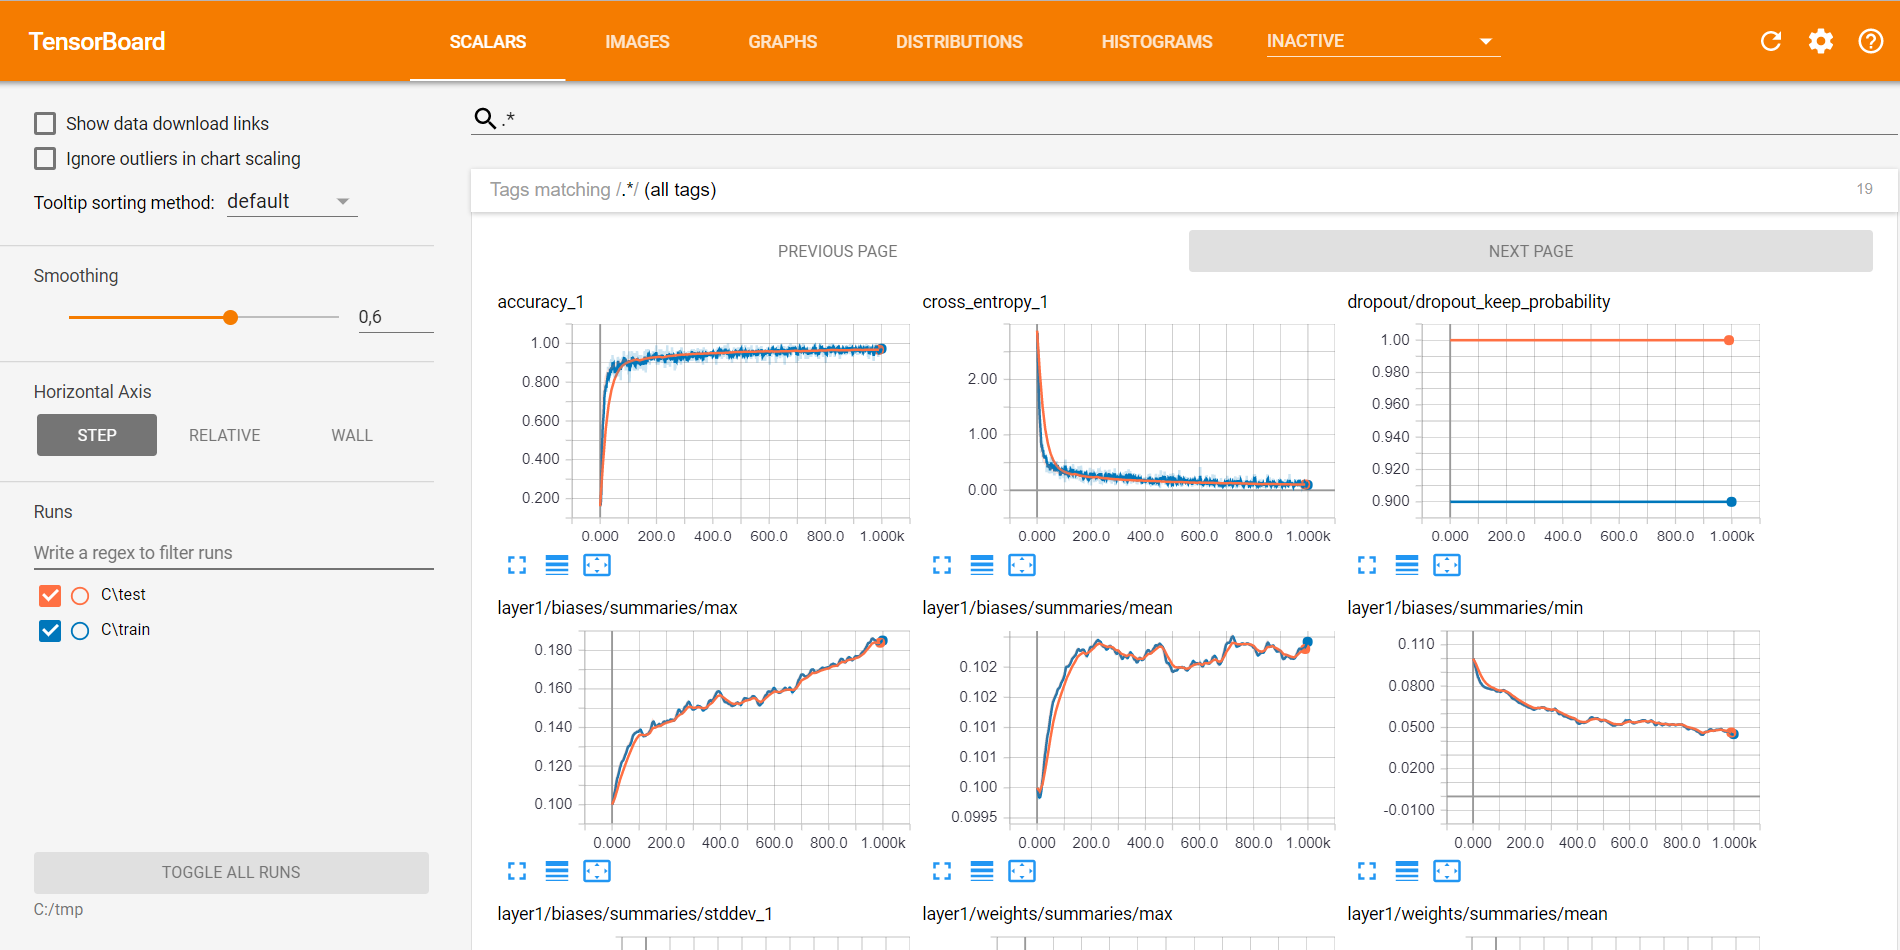
\includegraphics[width=1\textwidth]{images/Kapitel_3/TensorBoard_start.png}\\
	\vspace{10pt} 
	\caption[Die Startseite von TensorBoard]{Die Startseite von TensorBoard}
	\label{fig:tensorboard_start}
\end{figure}



\subsection{Die einzelnen Visualisierungsmöglichkeiten im Detail}

\textbf{\textit{Skalare}} 
\vspace{10pt}\\
Unter dem Reiter Skalare, welche mit der Klasse \dq tf.summary.scalar\grqq{}  abgespeichert werden, können verschiedenste Statistiken während eines Trainingsprozesses visualisiert werden. Dies könnten zum Beispiel die Genauigkeit oder Cross-Entropie sein, welche in Abbildung \ref{fig:skalare} dargestellt sind. Hierbei wird die Genauigkeit über den einzelnen Trainingsschritten aufgetragen. Wählt man mit der Maus einen bestimmten Datenpunkt aus, so werden zahlreiche weitere Informationen angezeigt. Ebenso ist hierbei ersichtlich, dass auch Trainings- und Testdaten gleichzeitig angezeigt und miteinander verglichen werden können.

\begin{figure}[h!]
	\centering
	%\vspace{-35pt}
	%\hspace{-1.0cm} 
	 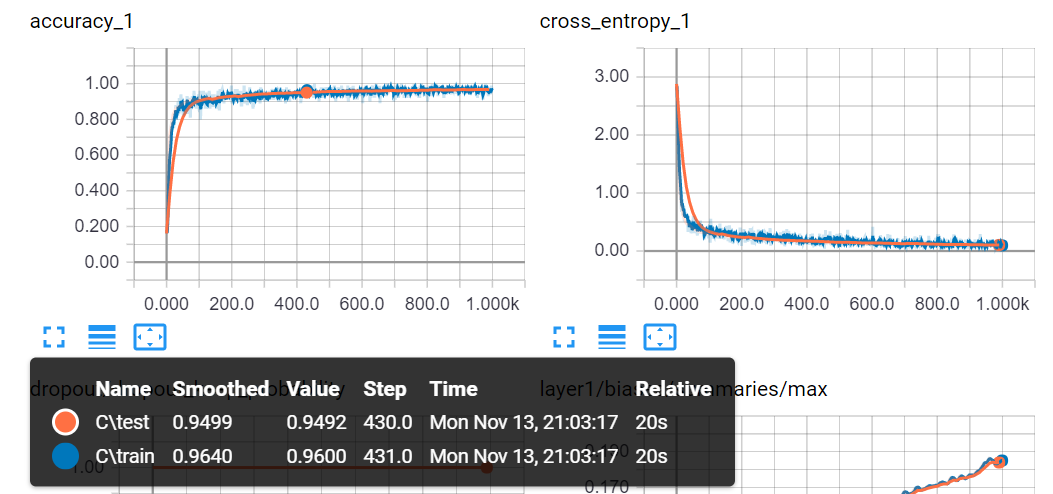
\includegraphics[width=0.8\textwidth]{images/Kapitel_3/skalars.png}\\
	\vspace{10pt} 
	\caption[Visualisierung der 'Accuracy' und 'Cross\_entropy' über die einzelnen Trainingsschritte]{Visualisierung der 'Accuracy' und 'Cross\_entropy' über die einzelnen Trainingschritte}
	\label{fig:skalare}
\end{figure}


\textbf{\textit{Bilder}}
\vspace{30pt}

\begin{wrapfigure}{r}{6cm}
	\vspace{-45pt}
	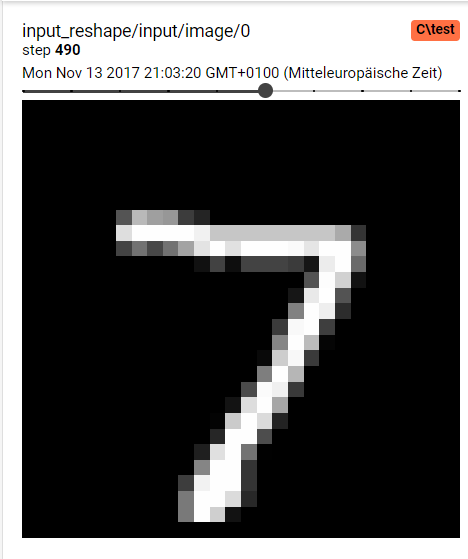
\includegraphics[width=6cm]{images/Kapitel_3/images.png}
	\caption{Bild des Testschrittes 490}
\end{wrapfigure}

Innerhalb des Reiters Bilder, welche mit der Klasse \dq tf.summary.image\grqq{} abgespeichert werden, können zur genaueren Analyse die Test- und Trainingsbilder eingesehen werden. 
Über den Bildern ist eine Scrollbar vorhanden mit dieser können einzelne Test- und Trainingsschritte ausgewählt werden, wodurch genau ersichtlich wird, welches Bild zum aktuellen Durchlauf gehört.
\vspace{50pt}
\newpage


\begin{figure}[t]
\begin{minipage}[t]{0.475\textwidth}
\centering
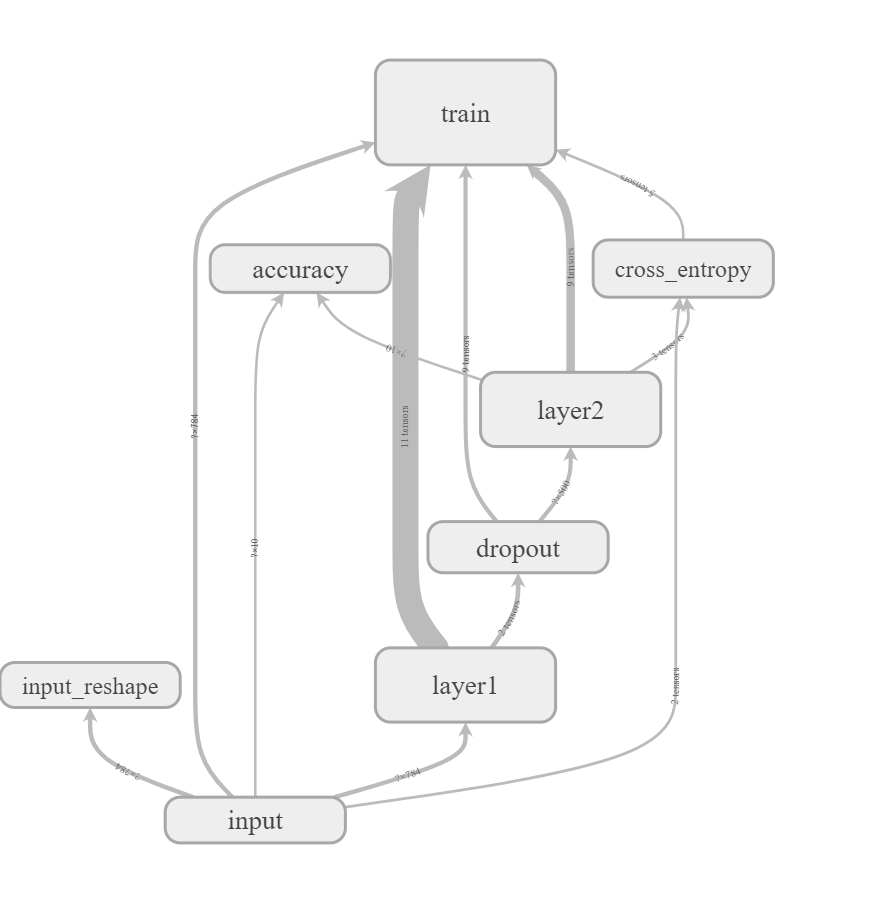
\includegraphics[width=0.9\textwidth]{images/Kapitel_3/graph.png}
\caption{TensorFlow Graph mit definierten Name scopes}
\label{fig:TensorFlow_Graph}
\end{minipage}
\hfill
\begin{minipage}[t]{0.475\textwidth}
\centering
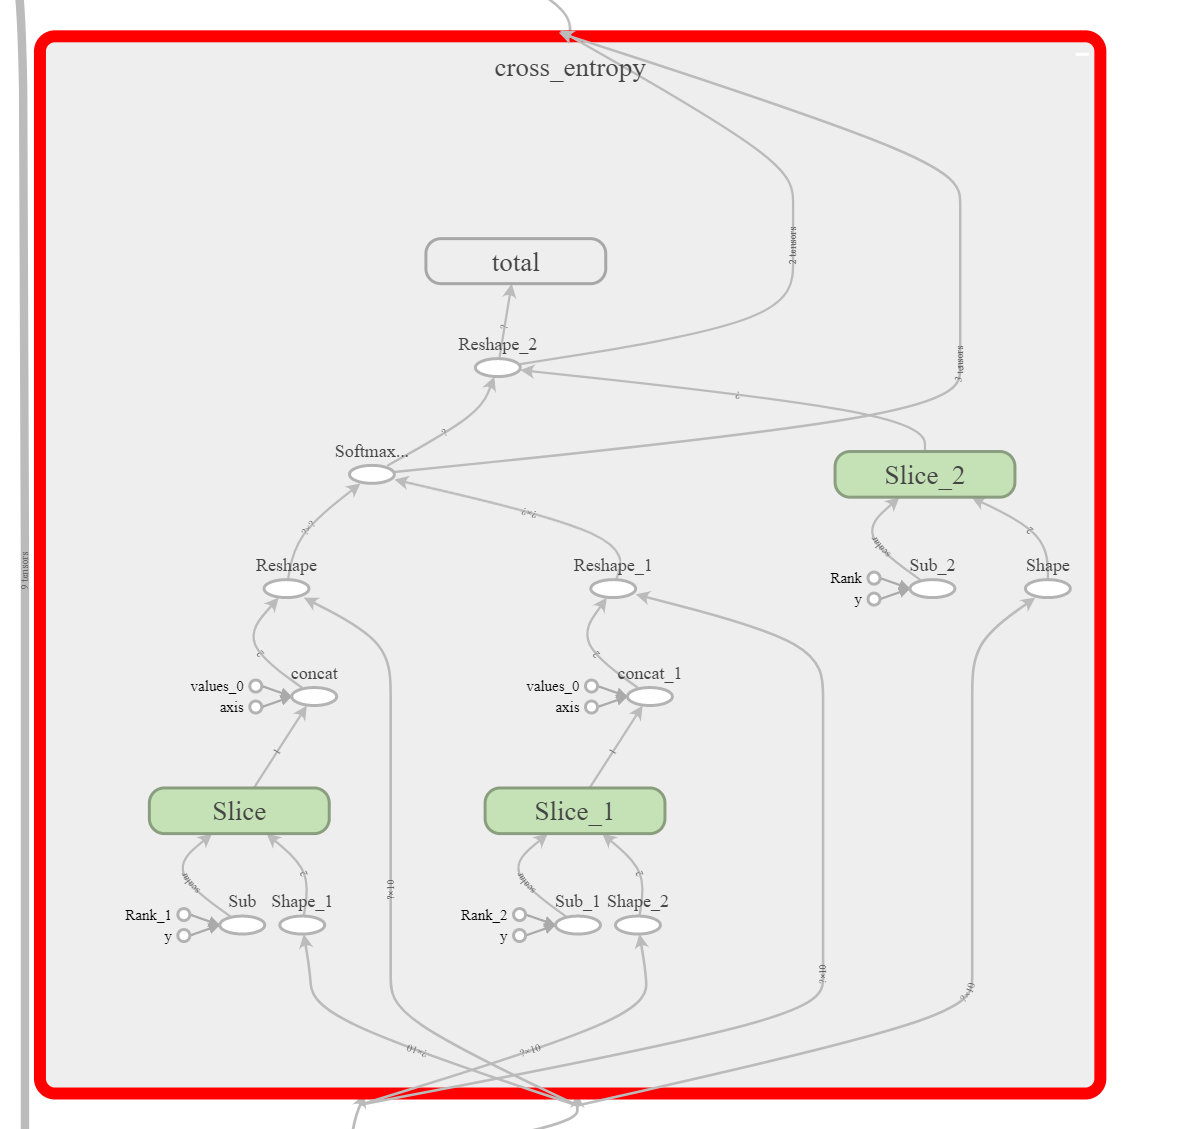
\includegraphics[width=0.9\textwidth]{images/Kapitel_3/graph1.png}
\caption{Name scope 'cross\_entropy' unterteilt in weiteren Operationen}
\label{fig:name_scope_cross_entropy}
\end{minipage}
\end{figure}

\textbf{\textit{Graphen}}
\vspace{10pt}\\
Unter dem Reiter Graphen befindet sich das komplette TensorFlow Model als Graph wie in Abbildung \ref{fig:TensorFlow_Graph} zu sehen ist. Um einen Graphen in Tensorboard zu erhalten, müssen im Programm die gewünschten Operationen als Name scope erstellt werden. Mit nachfolgendem Befehl \ref{formel3} erhält man einen 'cross\_entropy' Name scope: 


\begin{equation}
\displaystyle with \quad tf.name\_scope('cross\_entropy'):
\label{formel3}
\end{equation}

Der Name scope \textit{cross\_entropy} Abbildung \ref{fig:name_scope_cross_entropy} kann natürlich wiederum in mehrere Untergruppierungen aufgeteilt werden. So erhält man eine übersichtliche Visualisierung komplexer TensorFlow Modelle. 

\vspace{10pt}
\textbf{\textit{Histogramme}}
\vspace{10pt}\\
Unter dem Reiter Histogramme, welche mit der Klasse \dq tf.summary.histogram\grqq{} abgespeichert werden, wird die statistische Verteilung eines Tensors über der Zeit dargestellt. Im Histogramm sind zeitliche \dq Slices\grqq{} der Daten visualisiert, wobei jeder einzelne Slice ein Histogramm des Tensors in einem einzelnen Schritt darstellt. In Abbildung \ref{fig:histogram} ist ein einzelner Slice schwarz markiert.


\begin{figure}[h!]
	\centering
	%\vspace{-35pt}
	%\hspace{-1.0cm} 
	 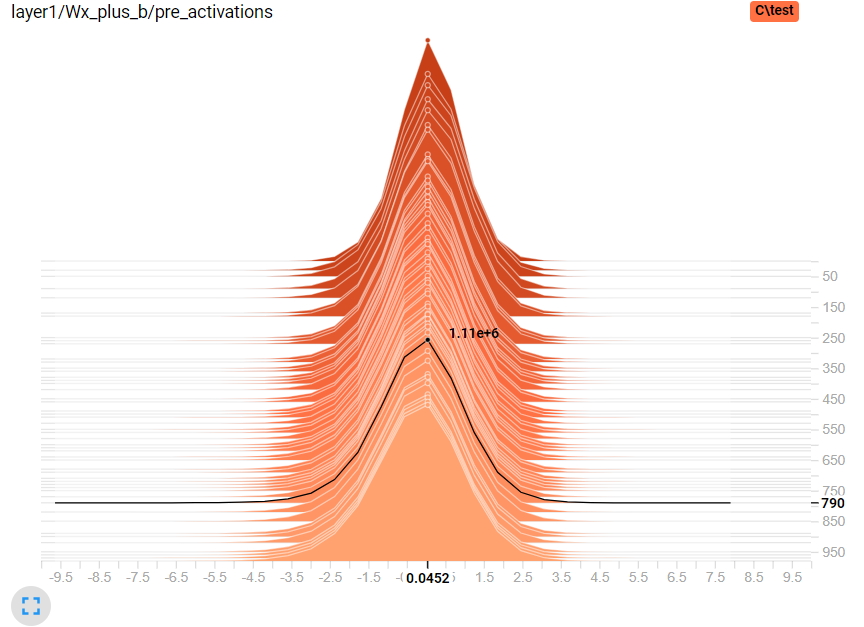
\includegraphics[width=0.7\textwidth]{images/Kapitel_3/histogram.png}\\
	\vspace{10pt} 
	\caption[Visualisierung eines Histogramms über die einzelnen Trainingsschritte]{Visualisierung eines Histogramms über die einzelnen Trainingschritte}
	\label{fig:histogram}
\end{figure}



\textbf{\textit{Verteilungen}}

\begin{center}
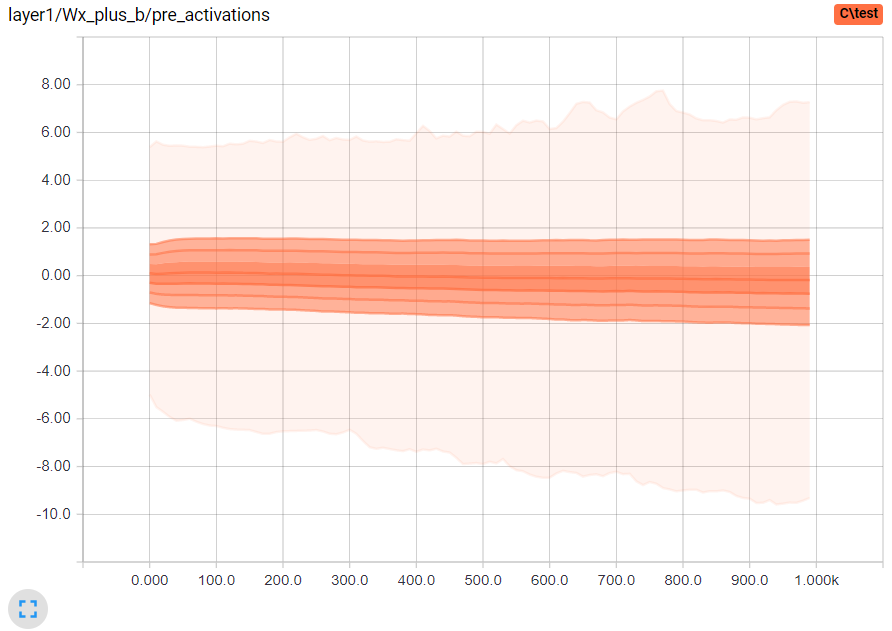
\includegraphics[width=0.6\textwidth]{images/Kapitel_3/distribution.png}
\end{center}


\textbf{\textit{Audio}}

\textbf{\textit{Projektor}}

\textbf{\textit{Text}}






\subsection{Die Graphelemente im Datenfluss}

 Dafür wurden zahlreiche unterschiedliche Elemente definiert, welche nachfolgend kurz erläutert werden. 
\\

\begin{tabular}{ p{4cm}p{10.8cm} ll }

\textbf{Namespace} \tabularnewline 
\includegraphics[width=0.1\textwidth]{images/Kapitel_3/namespace.png}
\label{fig:namespace}
 & High-level Knoten repräsentiert einen definierten Namensbereich.   \tabularnewline
  
\textbf{Unconnected series} \tabularnewline 

\includegraphics[width=0.1\textwidth]{images/Kapitel_3/Unconnected_series.png}
\label{fig:Unconnected_series}
 & Nummerierte Knoten, die nicht miteinander verbunden sind. \tabularnewline
  
\textbf{Connected series} \tabularnewline 

\includegraphics[width=0.1\textwidth]{images/Kapitel_3/Connected_series.png}
\label{fig:Connected_series}
 & Nummerierte Knoten, die miteinander verbunden sind. \tabularnewline 
 
\textbf{Operation node} \tabularnewline 

\includegraphics[width=0.1\textwidth]{images/Kapitel_3/Operation_node.png}
\label{fig:Operation_node}
 & Ein Knoten der eine einzelne Operation darstellt.  \tabularnewline 
 
\textbf{Constant} \tabularnewline 

\includegraphics[width=0.08\textwidth]{images/Kapitel_3/Constant.png}
\label{fig:Constant}
 & Repräsentiert eine Konstante im Programm.  \tabularnewline 

\textbf{Summary node} \tabularnewline 

\includegraphics[width=0.07\textwidth]{images/Kapitel_3/Summary_node.png}
\label{fig:Summary_node}
 & Dieser Knoten stellt eine Zusammenfassung dar.  \tabularnewline 

\textbf{Dataflow edge} \tabularnewline 

\includegraphics[width=0.1\textwidth]{images/Kapitel_3/Dataflow_edge.png}
\label{fig:Dataflow_edge}
 & Durchgezogener Pfeil zeigt den Datenfluss zwischen den Operationen an.  \tabularnewline
 
\textbf{Control edge} \tabularnewline 

\includegraphics[width=0.1\textwidth]{images/Kapitel_3/Control_dependency_edge.png}
\label{fig:Control_dependendy_edge}
 & Gepunkteter Pfeil zeigt die Steuerungsabhängigkeit zwischen den Operationen an.  \tabularnewline 
 
\textbf{Reference edge} \tabularnewline 

\includegraphics[width=0.1\textwidth]{images/Kapitel_3/Reference_edge.png}
\label{fig:Reference_edge}
 & Gelber Pfeil bedeutet, dass die ausgehende Operation die ankommende mutieren kann   \tabularnewline 
% & \tabularnewline
\end{tabular}
\\
